% !TEX TS-program = pdflatex
\documentclass[11pt]{article}
\usepackage[margin=1in]{geometry}
\usepackage{graphicx}
\usepackage{amsmath, amssymb}
\usepackage{authblk}
\usepackage{siunitx}
\usepackage[hidelinks]{hyperref}
\usepackage{csquotes}

% Bibliography with biblatex
\usepackage[backend=biber,style=authoryear,sorting=nyt,maxcitenames=2,maxbibnames=9]{biblatex}
\addbibresource{references.bib}

\title{A Computational Approach to Maximal Colour Perception Shift}
\author{Alex Grant}
\affil{Improbability Engineering}
\date{\today}

\begin{document}
\maketitle

\begin{abstract}
We present a computational method for identifying surround colours that cause the greatest perceptual shift in the appearance of a fixed stimulus colour. The method simulates perceptual colour appearance using the CIECAM02 model and quantifies differences in appearance with the CAM02-UCS metric $\Delta E_{\mathrm{UCS}}$. By comparing the perceived colour of a fixed stimulus across a large set of candidate surrounds, we identify surrounds that maximise the perceptual shift. This system offers a quantitative analogue to the contextual colour investigations pioneered by Josef Albers, and it provides an accessible tool for both creative practice and scientific study of contextual colour phenomena.
\end{abstract}

\section{Introduction}
The perceived colour of a stimulus is not determined solely by its physical properties but is deeply influenced by its surrounding context, a visual artefact arising from human cone responses and subsequent neural processing. This phenomenon underpins optical illusions and artistic practice, notably in the pedagogical experiments of Josef Albers \parencite{albers1963interaction}.

Here we develop a \emph{computational} approach to quantify and optimise context-driven perceptual shifts. Our goal is to identify ``Albers-extrema'': candidate surround colours that most dramatically alter the perceived appearance of a fixed stimulus colour relative to a reference surround. We show how colour appearance models and perceptual difference metrics can formalise this process.

\section{Background}
\subsection{Perceptual colour shift}
Visual responses are context-dependent: a central patch’s appearance depends on its surround via centre–surround mechanisms. Artists have long exploited this to create advancing, retreating, or vibrating colours. Albers’ \emph{Interaction of Color} \parencite{albers1963interaction} codified this in art pedagogy.

\subsection{Colour appearance models}
To model contextual influences, we use CIECAM02 \parencite{CIECAM02}, which accounts for luminance level, adaptation, and background colour. Its correlates are lightness $J$, colourfulness $M$, and hue $h$. For perceptual uniformity we map these to CAM02-UCS \parencite{fairchild2013color}, which defines approximately uniform coordinates $(J',a',b')$.

\subsection{Perceptual difference metrics}
In CAM02-UCS, Euclidean distance approximates perceived difference. Given two colours $(J'_1,a'_1,b'_1)$ and $(J'_2,a'_2,b'_2)$, their perceptual difference is
\begin{equation}
\Delta E_{\mathrm{UCS}} = \sqrt{(J'_1 - J'_2)^2 + (a'_1 - a'_2)^2 + (b'_1 - b'_2)^2}.
\end{equation}
This $\Delta E_{\mathrm{UCS}}$ serves as a quantitative proxy for visual distinctness. For comparison, the $\Delta E_{2000}$ metric is widely used for CIELAB \parencite{Luo2006}.

\section{Methods}
\subsection{Optimisation objective}
Given a fixed stimulus colour $C_{\text{stim}}$ and reference surround $C_{0}$, we compute its perceived appearance $P_{0}$ with CIECAM02. For each candidate surround $C_i$, the model yields $P_i$. The perceptual shift is
\begin{equation}
\Delta E_i = \lVert P_i - P_{0}\rVert_{\mathrm{UCS}}.
\end{equation}
The goal is to identify surrounds $C^*$ that maximise $\Delta E_i$.

\subsection{Centre–surround model}
We approximate surround effects using the chromatic adaptation and viewing-condition parameters of CIECAM02. The surround defines the adapting field luminance $L_A$, surround factor $F$, and white point reference, which determine the transformation of the fixed stimulus through the CAT02 chromatic adaptation transform. This yields context-dependent perceptual correlates.

\subsection{Implementation}
We implemented the algorithm in Python using the open-source \texttt{colour-science} package \parencite{colour-science}. Candidate surrounds are sampled from a uniform grid in sRGB; out-of-gamut colours are excluded. An optional perceptual similarity filter discards candidates with $\Delta E_{\mathrm{UCS}}$ below a user-specified threshold, ensuring that only distinct surrounds are considered. Users can also invert the search to identify stimulus colours most sensitive to context. Source code is available \parencite{colourshift}.

\section{Results and Examples}
\begin{figure}[h!]
\centering

\includegraphics[width=0.8\textwidth]{1.png}
\caption{Stimulus colour and original vs maximally shifting surround.}
\end{figure}

\begin{figure}[h!]
\centering

\includegraphics[width=0.8\textwidth]{2.png}
\caption{Second ranked alternate surround.}
\end{figure}

\begin{figure}[h!]
\centering

\includegraphics[width=0.8\textwidth]{3.png}
\caption{Third ranked alternate surround.}
\end{figure}

\begin{figure}[h!]
\centering
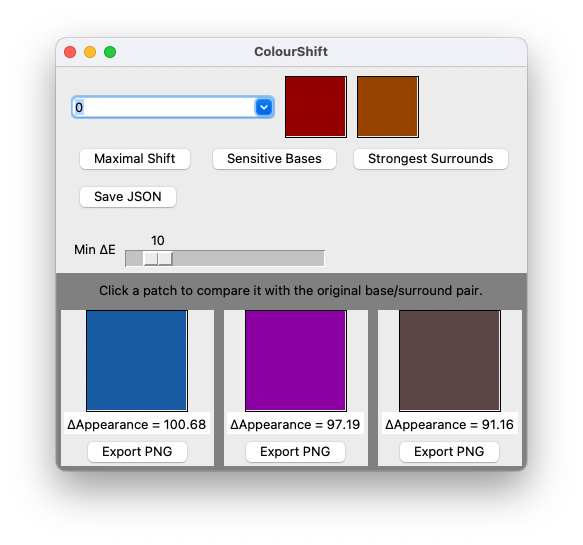
\includegraphics[width=0.8\textwidth]{screenshot.png}
\caption{Screenshot of the application interface showing stimulus, candidate surrounds, and calculated perceptual shifts.}
\end{figure}

\section{Discussion}
\paragraph{Applications.} This method formalises a long-standing artistic practice and extends it into quantitative territory. The results support colour design, accessibility considerations, and educational visualisation of colour relativity. For artists, the tool acts as a ``digital Albers exercise.''

\paragraph{Observations.} Early experiments suggest maximally shifting surrounds often exhibit complementary hues. Investigating the structure of these extrema vectors may reveal systematic relationships between stimulus and surround in perceptual space.

\paragraph{Limitations.} Model assumptions, observer variability, and display calibration constrain applicability. High-level cultural and semantic associations with colour are not captured by appearance models.

\section{Conclusion}
We introduced a computational method to identify surrounds that cause maximal perceptual change to a fixed stimulus. By combining colour appearance models and perceptual metrics, we provide a tool that connects scientific modelling with creative exploration.

\appendix
\section{Mathematical Formulation}
Let $XYZ_{\text{stim}}$ and $XYZ_{\text{surr}}$ denote tristimulus values of the stimulus and surround. The steps are:

\begin{enumerate}
  \item Compute adapting field luminance $L_A$ and surround factor $F$ from $C_{\text{surr}}$.
  \item Derive a reference white point from $C_{\text{surr}}$.
  \item Apply CAT02 chromatic adaptation to $XYZ_{\text{stim}}$.
  \item Run the full CIECAM02 model to obtain $(J,M,h)$.
  \item Convert $(J,M,h)$ to CAM02-UCS $(J',a',b')$.
\end{enumerate}

Thus the surround modulates visual adaptation, altering perceived appearance of the fixed stimulus.

\printbibliography

\end{document}
